\begin{tikzpicture}[
  x=1cm,
  y=1cm,
  >=Latex,
  flow/.style={->, thick, draw=black!75},
  feedback/.style={->, thick, draw=red!70!black},
  data/.style={draw=blue!65!black, fill=blue!12, rounded corners=2pt, align=center, minimum width=2.25cm, minimum height=0.62cm, inner sep=3pt},
  format/.style={draw=green!55!black, fill=green!12, rounded corners=2pt, align=center, minimum width=2.25cm, minimum height=0.62cm, inner sep=3pt},
  model/.style={draw=orange!75!black, fill=orange!18, rounded corners=2pt, align=center, minimum width=2.25cm, minimum height=0.62cm, inner sep=3pt},
  loss/.style={draw=red!65!black, fill=red!8, rounded corners=2pt, align=center, minimum width=2.25cm, minimum height=0.62cm, inner sep=3pt},
  panel/.style={draw=black!20, rounded corners=2pt, minimum width=3.88cm, minimum height=5.22cm, inner sep=0pt},
  every node/.style={font=\sffamily\scriptsize}
]
  % Shared data preparation
  \node[inner sep=0pt] (ct) at (0.72,0.90)
    {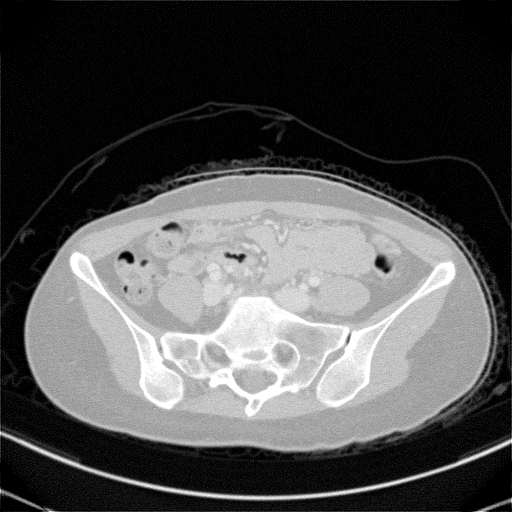
\includegraphics[width=0.95cm,height=0.95cm]{figures/ldct_example.png}};
  \node[font=\sffamily\tiny, align=center] (ct-label) at (0.72,0.16) {LDCT slice\\TIFF};
  \node[data, minimum width=1.45cm] (mos) at (2.30,0.90) {Radiologist\\MOS label};
  \node[data] (png) at (1.52,1.98) {Normalize intensity\\TIFF $\rightarrow$ PNG};
  \node[format] (jsonl) at (1.52,3.08) {Base JSONL record\\\texttt{image\_path}, \texttt{mos\_score}};
  \node[format] (arrow) at (1.52,4.16) {Arrow chat dataset\\messages, path, MOS};
  \draw[flow] (ct.north) -- (png.south west);
  \draw[flow] (mos.north) -- (png.south east);
  \draw[flow] (png) -- (jsonl);
  \draw[flow] (jsonl) -- (arrow);
  \node[panel] (prep-panel) at (1.52,2.38) {};

  % SFT branch
  \node[format, text width=2.82cm] (sft-row) at (5.56,4.16) {Chat row\\image + instruction\\+ target};
  \node[model] (sft-trl) at (5.56,2.82) {TRL \texttt{SFTTrainer}\\assistant-only loss};
  \node[model] (sft-model) at (5.56,1.60) {MedGemma 1.5\\+ LoRA adapter};
  \node[loss] (sft-out) at (5.56,0.34) {Generated target\\\texttt{\{"rating": y\}}};
  \draw[flow] (sft-row) -- (sft-trl);
  \draw[flow] (sft-trl) -- (sft-model);
  \draw[flow] (sft-model) -- (sft-out);
  \node[panel] (sft-panel) at (5.56,2.38) {};

  % GRPO branch
  \node[format] (grpo-row) at (9.60,4.16) {Prompt-only row\\image + instruction};
  \node[model] (grpo-trl) at (9.60,2.96) {TRL \texttt{GRPOTrainer}\\base or SFT initialization};
  \node[model] (grpo-gen) at (9.60,1.62) {MedGemma 1.5 + LoRA\\group of 4 completions};
  \node[loss] (grpo-reward) at (9.60,0.34) {MOS reward\\$R(\hat{y},y)=-|\hat{y}-y|$};
  \draw[flow] (grpo-row) -- (grpo-trl);
  \draw[flow] (grpo-trl) -- (grpo-gen);
  \draw[flow] (grpo-gen) -- (grpo-reward);
  \draw[feedback] (grpo-reward.east) -- ++(1.04,0) |- (grpo-trl.east);
  \node[panel] (grpo-panel) at (9.60,2.38) {};

  % Dataset routing across training modes
  \draw[flow] (arrow.north) -- ++(0,0.62) -| (sft-row.north);
  \draw[flow] (arrow.north) -- ++(0,0.62) -| (grpo-row.north);

  % Panel captions
  \node[font=\sffamily\scriptsize, align=center, text width=3.35cm] at (1.52,-0.78) {(a) LDCT data\\preparation};
  \node[font=\sffamily\scriptsize, align=center, text width=3.45cm] at (5.56,-0.78) {(b) Supervised\\fine-tuning};
  \node[font=\sffamily\scriptsize, align=center, text width=3.45cm] at (9.60,-0.78) {(c) GRPO\\refinement};
\end{tikzpicture}
